% =====================================================================
%  Frame "structured pruning".
%  Etait la seconde des deux frames de frames_tpu_pruning.tex.
% =====================================================================

\begin{frame}
\frametitle{Structured pruning}

\vspace{0.2cm}

{\small
\begin{itemize}\setlength{\itemsep}{7pt}
  \item[{\color{blue!80!black}$\bullet$}]
    There are \textbf{two types of pruning}:
    \begin{itemize}\setlength{\itemsep}{4pt}\setlength{\topsep}{4pt}
      \item[{\color{blue!80!black}--}]
        \emph{Unstructured}: weights become zeros, tensor shapes do not change.
      \item[{\color{blue!80!black}--}]
        \emph{Structured}: whole filters are removed, so the tensors really get
        smaller and the model really gets faster.
        \textbf{We choose this one.}
    \end{itemize}
  \item[{\color{blue!80!black}$\bullet$}]
    The added difficulty is \textbf{dependency tracking}: cutting one filter
    changes the layers it feeds, and residual additions or concatenations tie
    several layers together. All of them must be cut consistently.
  \item[{\color{blue!80!black}$\bullet$}]
    Filters are ranked \textbf{across the whole network}: we set one target for
    the model, and the rate of each layer follows from the ranking.
\end{itemize}}

\vspace{0.3cm}
\begin{center}
\makebox[\linewidth][c]{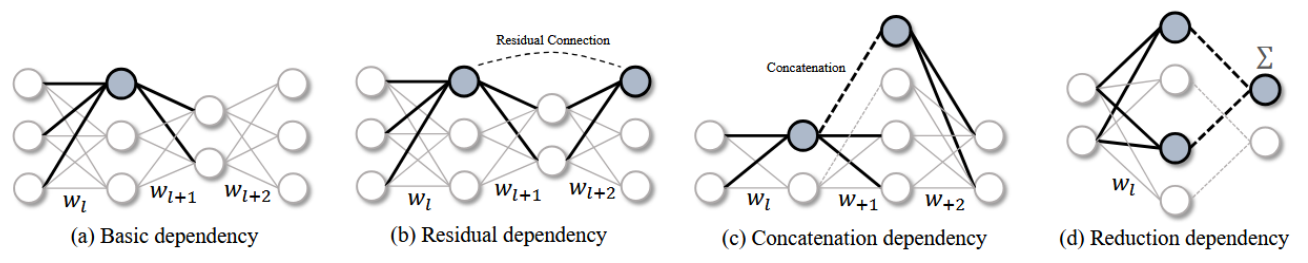
\includegraphics[width=1.0\linewidth]{bench/img/dependencies.png}}
\end{center}

\end{frame}
